\documentclass{article}
\usepackage{tikz}
%-----------------------
% Document information
%-----------------------


\title{Statistic Stuffs}

\author{Roberto \textsc{Antoniello}}

\begin{document}

\maketitle

\begin{center} I will drop here some statistic concepts I liked during the course I had at University of Milan.\end{center}

\section{Gini index}

There are two types of Gini indexes. One has the purpose of telling how much a sample is heterogeneous. The other one is used for concentration. We will talk about the first one we have mentioned and is defined as follow:
\begin{center}$$I = 1 - \sum_{j=1}^{k}f_j^2$$\end{center}

This index is always less than 1 and always more than 0.

\begin{center}$0 \leq I < 1$\end{center}

So we are subtracting the squared relative frequencies from one. 

we know that: 
\begin{center}$$\forall j f_j \ge 0 \longrightarrow \sum_{j=1}^k f_j = 1$$.\end{center}

This implies that $\exists \acute{j} : \acute{f_j} > 0 \longrightarrow f_j^2 > 0$.

So: \begin{center}$$\sum_{j=1}^k f_j^2 > 0 \longrightarrow I < 1$$ as said in before.\end{center}

We can consider also that: $$\sum_{j=1}^kf_j^2 \le \sum_{j=1}^kf_j$$.

This implies that $$1 - \sum_{j=1}^kf_j^2 \ge 0$$.

We have just demonstrated what we said a few moments ago. $0 \leq I < 1$.  

\section{Probability calculus}

Before we can talk about probability, we have to define a probability function. So we need to define as first $\Omega$ as the set of all possibles outcomes. Then we can say what is an event, which is just a subset of $\Omega$. Now let's define what is an Event algebra:
$$\mathcal{A} = \left\{E_i \subseteq \Omega\right\}$$
$E_i$ are all the subsets events in $\Omega$. This algebra has to respect three rules:

1. $\Omega \in \mathcal{A}$

2. $\forall E \subseteq \Omega \longrightarrow E \in \Omega \rightarrow \bar E \in \Omega$

3. $\forall E,F \subseteq \Omega \longrightarrow E \in \mathcal{A}, F \in \mathcal{A} \rightarrow E \cup F \in \mathcal{A}$

The third rule can be extended to this: $$\forall i=1,2,..,n E_i \subseteq \Omega, E_i \in \mathcal{A} \rightarrow \bigcup_{i=1}^nE_i \in \mathcal{A}$$

Finally we can define the probability function.

$P  :  \mathcal{A} \rightarrow \mathbb{R}$

\subsection{Kolmogorov axioms}

Kolmogorov axioms are the fundamental rules of the probability calculus.

A1. $\forall E \in \mathcal{A} \ \ 0 \leq P(E) \leq 1$

A2. $P(\Omega) = 1$

A3. $\forall E_1...E_n \ \ \forall i \ E_i \in \mathcal{A}$ mutually exclusive $\rightarrow P(\bigcup_{i=1}^nE_i) = \sum_{i=1}^nP(E_i)$

\subsection{Elemental theorems of Probability}

1. First theorem

$\forall E \in \mathcal{A} \ \ \ P(\bar E) = 1 - P(E)$
\bigskip

Demonstration:

We know that $1 = P(\Omega)$ from the second kolmogorov axiom.

We know also that $E \cap \bar E = \emptyset$ and that $E \cup \bar E = \Omega$

So:

$1 = P(\Omega) \rightarrow 1 = P(E \cup \bar E)$

Now we can use the third kolmogorov axiom and:

$1 = P(E) + P(\bar E) \rightarrow P(\bar E) = 1 - P(E)$

Demonstrated.
\bigskip

2. Second theorem

$\forall E,F \in \mathcal{A} \ \ \ P(E \cup F) = P(E) + P(F) - P(E \cap F)$
\bigskip

Demonstration:

Let's draw a Venn diagram to make it easier.

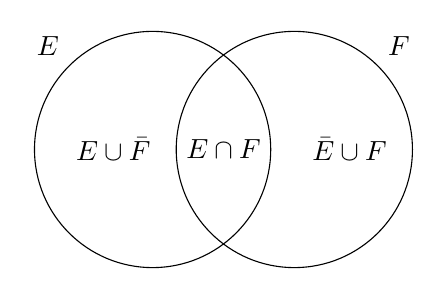
\begin{tikzpicture}
\node [draw,circle,minimum size = 3cm,label={135:$E$}] (E) at (0,0){}; %Set E
\node [draw,circle,minimum size = 3cm,label={45:$F$}] (F) at (1.8,0){}; %Set !F
\node at (0.9,0) {$E \cap F$};
\node at (-0.5,0) {$E \cup \bar F$};
\node at (2.5,0) {$\bar E \cup F$};

\end{tikzpicture}

We can get that $E \cup F = (E \cap \bar F) \cup (E \cap F) \cup (\bar E \cap F)$

So: $P(E \cup F) = P((E \cap \bar F) \cup (E \cap F) \cup (\bar E \cap F))$

Now we use again the third kolmogorov axiom:

$P(E \cup F) = P(E \cap \bar F) + P(E \cap F) + P(\bar E \cap F)$

But now we can transform $P(E \cap \bar F) + P(E \cap F)$ in $P(E)$ 

$P(E \cup F) = P(E) + P(\bar E \cap F)$

We need also $P(F)$, so I add and substract $P(E \cap F)$ which doesn't change anything.

$P(E \cup F) = P(E) + P(\bar E \cap F) + P(E \cap F) - P(E \cap F)$

And so we finished it because the result from getting $P(F)$ is:

$P(E \cup F) = P(E) + P(F) - P(E \cap F)$

Demonstrated.
\bigskip

3. Third theorem

$P(\emptyset) = 0$
\bigskip

Demonstration:

$P(\Omega) = 1$

we know from the first theorem that: $P(\bar E) = 1 - P(E)$

$P(\emptyset) = P(\bar \Omega) = 1 - P(\Omega) = 0$

Demonstrated.

\section{Total probability theorem and Bayes Theorem}

these two theorems can be useful to calculate complex probability by calculating more probabilities that are more simple.

\subsection{Total probability theorem(General form)}

Hypothesis:
\bigskip

A partition of $\Omega \longrightarrow F_1,F_2,...,F_n \subseteq \Omega$ 

$\forall i P(F_i) \neq 0$
\bigskip

Thesis:
$$P(E) = P(\bigcup_{i=1}^n (E \cap F_i)) = \sum_{i=1}^n P(E \cap F_i) = \sum_{i=1}^nP(E|F_i)\cdot P(F_i)$$

Where $P(A|B)$ is a conditional probability defined as follow:

$$P(A|B) = \frac{P(A \cap B)}{P(B)}$$

And from this last definition we say $P(A \cap B) = P(A|B) \cdot P(B)$ 

\subsection{Bayes Theorem}

The hypothesis are the same of the Total probability theorem(General form).
\bigskip

Thesis:

$$P(F_j|E) = \frac{P(F_j \cap E}{P(E)} = \frac{P(E|F_j)\cdot P(F_j)}{\sum_{i=1}^n P(E|F_i) \cdot P(F_i)}$$


From this theorem it's possible to build a classifier that is called Naive Bayes, which allow to simplify the calculus of some probability by using a naive hypothesis. We will not define this classifier here.

\section{Random variable}

A random variable is a function defined as follow:

$$X : \Omega \rightarrow \mathbb{R}$$

Or, if we want to be more precise:

$$\left\{X = \alpha\right\} \equiv \left\{\omega \in \Omega : X(\omega) = \alpha\right\}$$

Basically it's a function that associates a number to each outcome of a random experiment. We define the support as the set of all possible values that a random variable X can assume. 

In this document we will see discreet and continuous random variables.
\bigskip

The tools and graphics to work with random variables will be defined in a Jupyter notebook inside this repo.

\section{Markov and Tchebyshev inequalities}

These inequalities are interesting theoretic results we can use to give a esteem of a probability.
\bigskip

\subsection{Markov inequality}

Theorem:
\bigskip

$$X \geq 0 \ \ \  \forall a > 0 \rightarrow P(X \geq a) \leq \frac{\mathcal E(X)}{a}$$
\bigskip
Demonstration:

$$\mathcal E(X) = \int_{0}^{+ \infty} x \cdot f_x(x)dx = \int_{0}^ax\cdot f_x(x)dx + \int_{a}^{+ \infty} x \cdot f_x(x)dx \geq \int_{a}^{+ \infty} x \cdot f_x(x)dx$$

\bigskip 

$$\geq \int_{a}^{+ \infty} a \cdot f_x(x)dx = a \cdot \int_{a}^{+ \infty} f_x(x)dx = a \cdot P(X \geq a) \longrightarrow \mathcal E(X) \geq a \cdot P(X \geq a)$$

Now we divide both by a and it's demonstrated.

\subsection{Tchebyshev inequality}

We consider a random variable $X$ with $\mathcal E(X) = \mu$ and $Var(X) = \sigma^2$

Thesis:
$$\forall r > 0 \ \ P(|X - \mu| \geq r) \leq \frac{\sigma^2}{r^2}$$
\bigskip

Demonstration:

$|X - \mu| \geq r \leftrightarrow (X - \mu)^2 \geq r^2$
\bigskip

$P(|X - \mu| \geq r) = P((X - \mu)^2 \geq r^2)$

Let' define $$Y:= (X - \mu)^2 \rightarrow using \ markov \ P(Y \geq r^2) \leq \frac{\mathcal E(Y)}{r^2}$$

$$= \frac{\mathcal E((X- \mu)^2)}{r^2} = \frac{Var(X)}{r^2} = \frac{\sigma^2}{r^2}$$

Demonstrated.

\section{Random variables Models}

Models are useful to solve common problems with a common plan.

\subsection{Bernoulli model}

The bernoulli model describes the most simple experiment such as coin launch and similar. Every experiments have only two outcomes: success or failure.
\bigskip

$X \sim B(p) \ \ \ D_x = \left\{0,1\right\} \ \ \ p \in [0,1]$
\bigskip

$p_x(x) = P(X=x) = p^x \cdot(1-p)^{1-x} \cdot I_\left\{0,1\right\}^{(x)}$

= $1-p$ if $x = 0$ 

= $p$ if $x = 1$

= 0 otherwise
\bigskip

$\mathcal E(X) = p = \sum_{i}x_i P(X=xi)$

$Var(X)=p(1-p)$

\subsection{Binomial model}

This model is obtained from the Bernoulli by doing n bernoulli experiments with the same p parameter and with independence from each other. The variable counts the number of success.

$X \sim B(n,p) D_x = \left\{0,1,...,n\right\}$
\bigskip

$p_x(i) = P(X=i) = \left(\begin{array}{c} n \\ i \end{array} \right) \cdot p^i \cdot (1-p)^{n-i}\cdot I_\left\{D_x\right\}^{(x)}$
\bigskip

$$\mathcal E(X) = \mathcal(\sum_{i=1}^n X_i) = \sum_{i=1}^n \mathcal E(X) = \sum_{i=1}^n p = np$$

$$Var(X) = Var(\sum_{i=1}^n X_i) = \sum_{i=1}^nVar(X_i) = \sum{i=1}^np(1-p) = np(1-p)$$
\bigskip

If we have two binomial indipendent random variables with the same p but different n and we sum them we obtain this:

$$X_1 \sim B(n,p) \ and \ X_2 \sim B(m,p) \rightarrow X_1 + X_2 = Y \sim B(n+m,p)$$


\subsection{Discreet uniform model}

This model is used for experiments such as dice launch.

$X \sim U(n) D_x = \mathbb{N} \cup \left\{0\right\}$

$$p_x(i) = P(X = i) = \frac{1}{n} \cdot I_\left\{1,...,n\right\}^(i)$$
\bigskip

$$\mathcal E(X) = \frac{n+1}{2}$$

$$Var(X) = \frac{n^2 +1}{12}$$

The dispersion around the $\mathcal E(X)$ increase with the number of equal-probability events.


\subsection{Geometric Model}

This model is obtained from the Bernoulli by doing experiments and stop only when it comes the first success. The variable counts the number of failures before the first success. 
\bigskip

$X \sim G(p) \ \ p \in (0,1]$

$p_x(i) = P(X=i) (1-p)^i p \cdot I_{\mathbb{N} \cup {0}^(i)}$
\bigskip

$\mathcal E(X) = \frac{1-p}{p}$

$Var(X) = \frac{1-p}{p^2}$
\bigskip

This model has the property of Memorylessness, which is defined as follow:

$P(X \geq i + j| X \geq i) = P(X \geq j)$

The number of failures is saying nothing about the next experiment, the probability is the same.

\subsection{Poisson model}
work in progress


\end{document}
